\subsection{Definition}
%
Theis' problem examines the transient lowering of the water table induced by a pumping well. Theis' fundamental insight was to recognize that Darcy's law is analogous to the law of the heat flow by conduction, i.e., hydraulic pressure being analogous to temperature, pressure-gradient to thermal gradient.
%
The assumptions required by the Theis solution are:
\begin{itemize}
    \item the aquifer is homogeneous, isotropic, confined, infinite in radial extent,
    \item the aquifer has uniform thickness, horizontal piezometric surface
    \item the well is fully penetrating the entire aquifer thickness,
    \item the well storage effects can be neglect, 
    \item the well has a constant pumping rate,
    \item no other wells or long term changes in regional water levels. 
\end{itemize}
%
\subsection{Solution}
The analytical solution of the drawdown as a function of time and distance is expressed by Eq. ~\ref{theis}:
%
\begin{eqnarray}
h_0 - h(t,x,y) = \frac{Q}{4\pi T}W(u)
\label{theis}
\end{eqnarray}
%
\begin{eqnarray}
u = \frac{(x^{2}+y^{2})S}{4Tt}
\label{theis_u}
\end{eqnarray}
%
where $h_0$ is the constant initial hydraulic head $[L]$, $Q$ is the constant discharge rate [$L^{3}T^{-1}$], $T$ is the aquifer transmissivity [$L^{2}T^{-1}$], $t$ is time $[T]$, $x,y$ is the coordinate at any point $[L]$, $S$ is the aquifer storage $[-]$. $W(u)$ is the well function defined by an infinite series for confined aquifer as

\begin{eqnarray}
W(u) = \int^{+\infty}_{u} \frac{e^{-u}}{u} du = -\gamma -lnu + \sum^{\infty}_{k=1}{\frac{(-1)^{k+1}u^k}{k\cdot k!}}
\label{theis_wu}
\end{eqnarray}

where $\gamma\approx$ 0.5772 is the Euler-Mascheroni contant. For practical purposes, the simplest approximation of $W(u)$ was proposed as $W(u)=-0.5772-lnu$  for $u <$ 0.05. Other more exact approximations of the well function were summarized by R. Srivastava and A. Guzman-Guzman \cite{GWAT:GWAT844}.

The parameters and initial $\&$ boundary conditions are defined in Table.~\ref{1dTheis}.

\begin{table}[htb]
\caption{The parameters defined in 1-D Theis' problem.}
\centering
\begin{tabular*}{0.9\textwidth}{@{\extracolsep{\fill}}llrr}
\hline\noalign{\smallskip}
{Symbol} &{Parameter}& {Value} & {Unit} \\ 
\hline\noalign{\smallskip}
 $h(0,r)$  & Initial conditions & 0 & $m$  \\
 $Q$   & Well pumping rate      & 1.2233$\times 10^{3}$ & $m^{3}/d$  \\
 $h(t,304.8) $ & Boundary conditions  &0 & $m$  \\
  \hline\noalign{\smallskip}
 $K$ & Hydraulic conductivity & 9.2903$\times 10^{-4}$ & $m/s$  \\
 $S$ & Storage coefficient & 0.0010& -   \\
 $r$&0.3048 & Wellbore radius &  $m$ \\
  \noalign{\smallskip}\hline
\end{tabular*}
\label{1dTheis}
\end{table}
%
\begin{figure} [htb]
 \centering
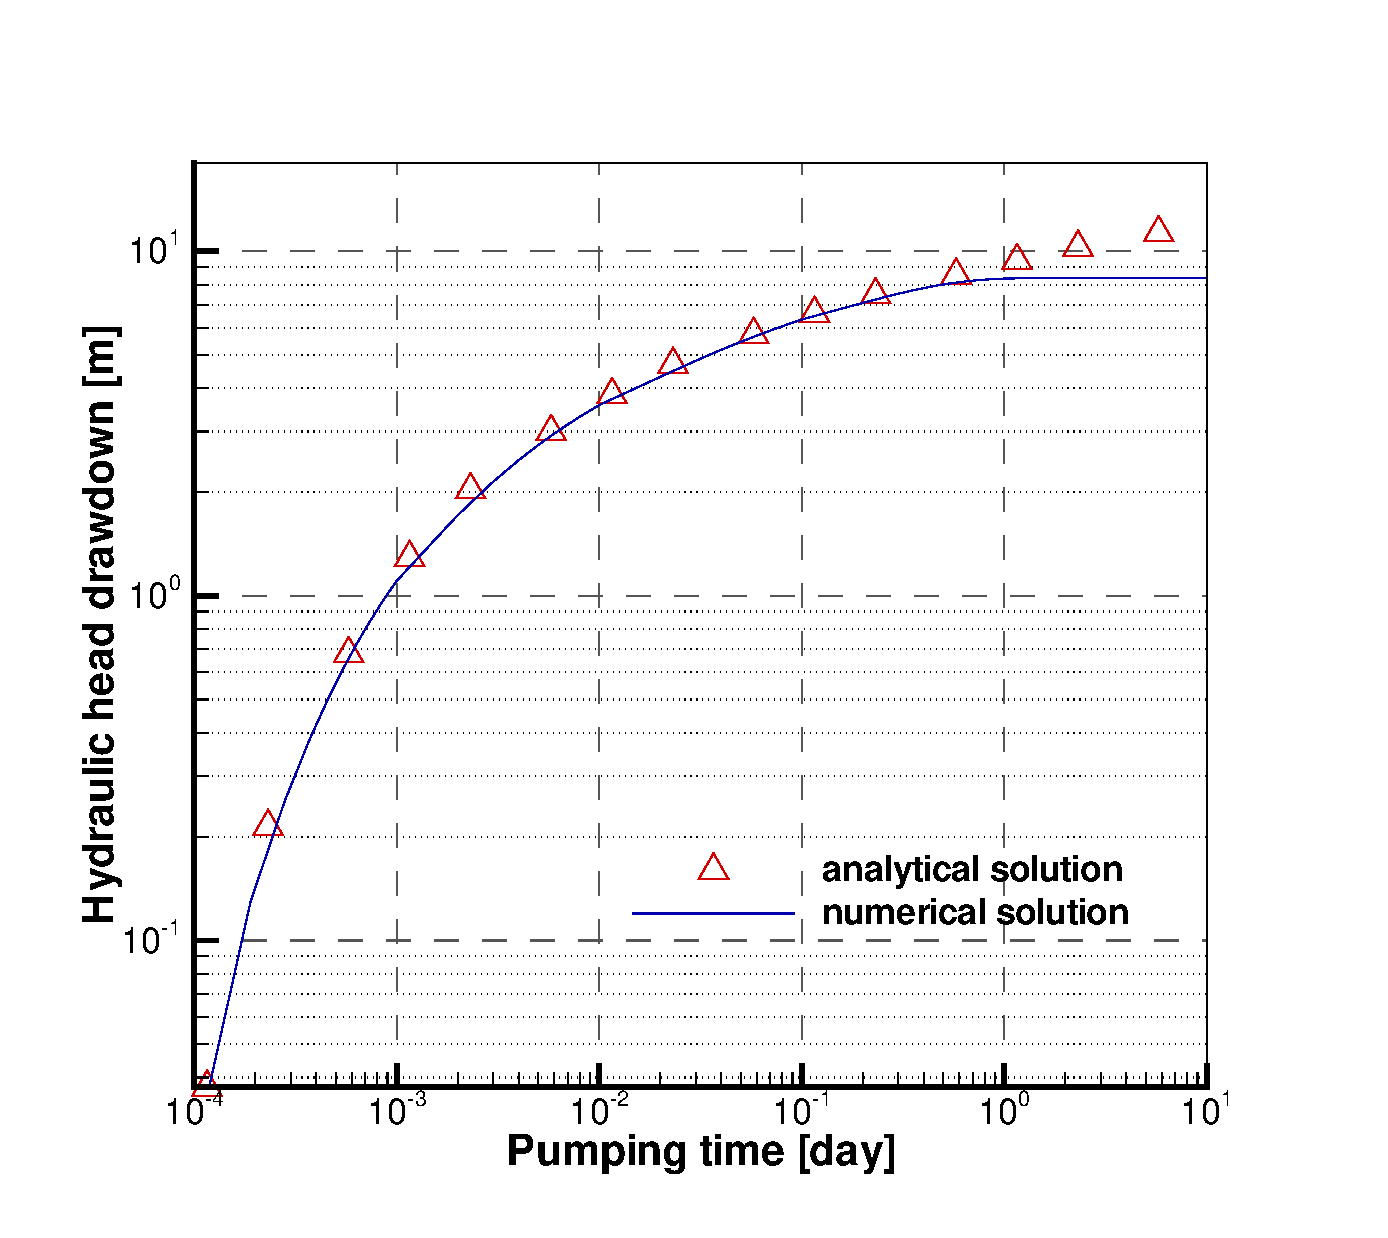
\includegraphics[width=0.7\columnwidth] {Chapter5/figure/Theis1.eps}
\caption{Calculated drawdowns at a distance of 9.639~m from the well.}
 \label{Theis1}
\end{figure}
%
%
\subsection{Results}
Fig.~\ref{Theis1} shows the comparison of analytically and numerically calculated drawdown of hydraulic head versus time at the distance of 9.639 m from the well.
%
\subsection{2-D application}
%
The 2-D application is solved in the following situation (Table.~\ref{2dTheis}).\\
%
\begin{table}[htb]
\centering
\caption{The parameters defined in 2-D Theis' problem.}
\begin{tabular*}{0.9\textwidth}{@{\extracolsep{\fill}}llrr}
\hline\noalign{\smallskip}
{Symbol}&{Parameter} & {Value} & {Unit} \\ 
\hline\noalign{\smallskip}
 $Q$ & Discharge rate       &  1000  				        & $m^{3}/d$  \\
 $S$ & Specific storage     &  $1.0\times 10^{-5}$	& $1/m$ \\
 $T$ &  Transmissivity      & 1000 				        & $m^{2}/d$ \\
 $B$ & Thickness of aquifer &  20 					        & $m$ \\
  \noalign{\smallskip}\hline
\end{tabular*}
\label{2dTheis}
\end{table}

The aquifer horizontal domain size is 1000~m $\times$ 750~m with the pumping well at the location coordinate (500, 375). The discretization of space is 10~m $\times$ 10~m grid. The simulation time is 151.2 seconds and the time step is 1.036 seconds. The initial head is 20~m in the whole domain and the boundary condition is 0~m drawdown at the left and right boundaries. There is no flux through the top and bottom boundaries. The cone of depression induced by the pumping well at the end of the simulation is plotted in Fig.~\ref{theis2}.

\begin{figure} [htb]
 \centering
 \vspace{-40pt}
 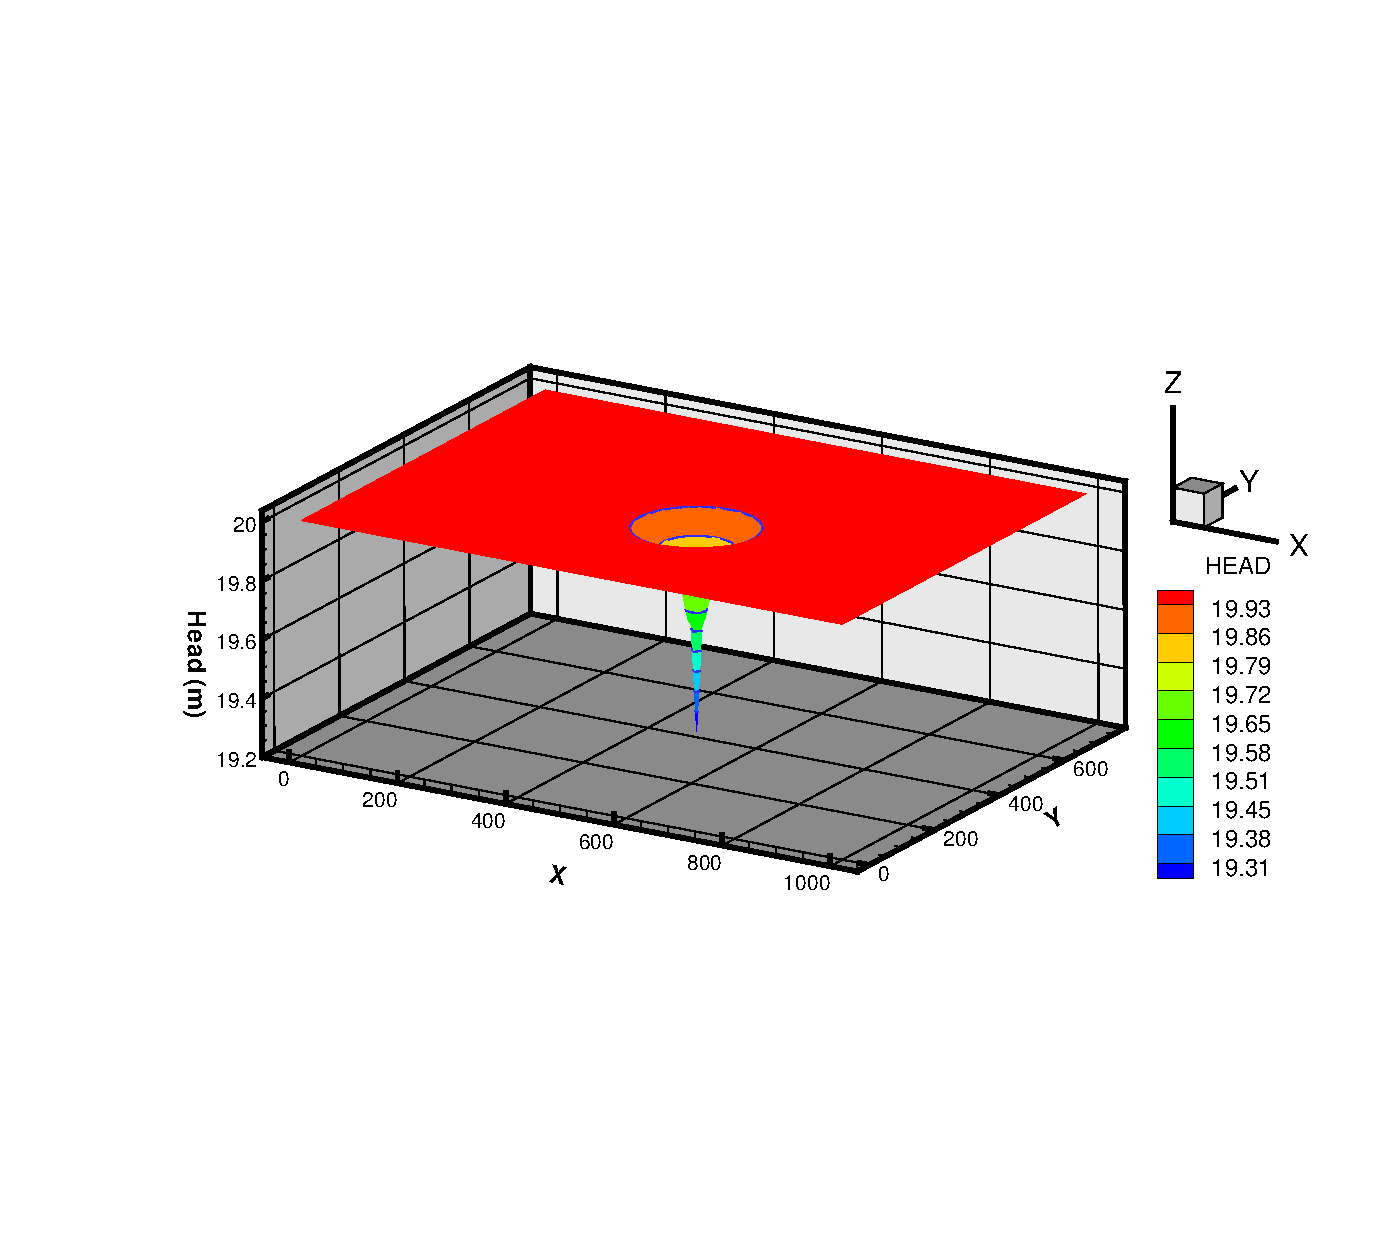
\includegraphics[width=1.0\columnwidth] {Chapter5/figure/Theis2.eps}
 \vspace{-50pt}
 \caption{Cone of depression at the end of the simulation.}
 \vspace{-20pt}
 \label{theis2}
\end{figure}